\documentclass{ximera}
\author{Jim Talamo \and Bart Snapp}
%\usepackage{todonotes}

\newcommand{\todo}{}

\usepackage{esint} % for \oiint
\ifxake%%https://math.meta.stackexchange.com/questions/9973/how-do-you-render-a-closed-surface-double-integral
\renewcommand{\oiint}{{\large\bigcirc}\kern-1.56em\iint}
\fi


\graphicspath{
  {./}
  {ximeraTutorial/}
  {basicPhilosophy/}
  {functionsOfSeveralVariables/}
  {normalVectors/}
  {lagrangeMultipliers/}
  {vectorFields/}
  {greensTheorem/}
  {shapeOfThingsToCome/}
  {dotProducts/}
  {partialDerivativesAndTheGradientVector/}
  {../productAndQuotientRules/exercises/}
  {../normalVectors/exercisesParametricPlots/}
  {../continuityOfFunctionsOfSeveralVariables/exercises/}
  {../partialDerivativesAndTheGradientVector/exercises/}
  {../directionalDerivativeAndChainRule/exercises/}
  {../commonCoordinates/exercisesCylindricalCoordinates/}
  {../commonCoordinates/exercisesSphericalCoordinates/}
  {../greensTheorem/exercisesCurlAndLineIntegrals/}
  {../greensTheorem/exercisesDivergenceAndLineIntegrals/}
  {../shapeOfThingsToCome/exercisesDivergenceTheorem/}
  {../greensTheorem/}
  {../shapeOfThingsToCome/}
  {../separableDifferentialEquations/exercises/}
  {vectorFields/}
}

\newcommand{\mooculus}{\textsf{\textbf{MOOC}\textnormal{\textsf{ULUS}}}}

\usepackage{tkz-euclide}
\usepackage{tikz}
\usepackage{tikz-cd}
\usetikzlibrary{arrows}
\tikzset{>=stealth,commutative diagrams/.cd,
  arrow style=tikz,diagrams={>=stealth}} %% cool arrow head
\tikzset{shorten <>/.style={ shorten >=#1, shorten <=#1 } } %% allows shorter vectors

\usetikzlibrary{backgrounds} %% for boxes around graphs
\usetikzlibrary{shapes,positioning}  %% Clouds and stars
\usetikzlibrary{matrix} %% for matrix
\usepgfplotslibrary{polar} %% for polar plots
\usepgfplotslibrary{fillbetween} %% to shade area between curves in TikZ
%\usetkzobj{all}
\usepackage[makeroom]{cancel} %% for strike outs
%\usepackage{mathtools} %% for pretty underbrace % Breaks Ximera
%\usepackage{multicol}
\usepackage{pgffor} %% required for integral for loops



%% http://tex.stackexchange.com/questions/66490/drawing-a-tikz-arc-specifying-the-center
%% Draws beach ball
\tikzset{pics/carc/.style args={#1:#2:#3}{code={\draw[pic actions] (#1:#3) arc(#1:#2:#3);}}}



\usepackage{array}
\setlength{\extrarowheight}{+.1cm}
\newdimen\digitwidth
\settowidth\digitwidth{9}
\def\divrule#1#2{
\noalign{\moveright#1\digitwidth
\vbox{\hrule width#2\digitwidth}}}




% \newcommand{\RR}{\mathbb R}
% \newcommand{\R}{\mathbb R}
% \newcommand{\N}{\mathbb N}
% \newcommand{\Z}{\mathbb Z}

\newcommand{\sagemath}{\textsf{SageMath}}


%\renewcommand{\d}{\,d\!}
%\renewcommand{\d}{\mathop{}\!d}
%\newcommand{\dd}[2][]{\frac{\d #1}{\d #2}}
%\newcommand{\pp}[2][]{\frac{\partial #1}{\partial #2}}
% \renewcommand{\l}{\ell}
%\newcommand{\ddx}{\frac{d}{\d x}}

% \newcommand{\zeroOverZero}{\ensuremath{\boldsymbol{\tfrac{0}{0}}}}
%\newcommand{\inftyOverInfty}{\ensuremath{\boldsymbol{\tfrac{\infty}{\infty}}}}
%\newcommand{\zeroOverInfty}{\ensuremath{\boldsymbol{\tfrac{0}{\infty}}}}
%\newcommand{\zeroTimesInfty}{\ensuremath{\small\boldsymbol{0\cdot \infty}}}
%\newcommand{\inftyMinusInfty}{\ensuremath{\small\boldsymbol{\infty - \infty}}}
%\newcommand{\oneToInfty}{\ensuremath{\boldsymbol{1^\infty}}}
%\newcommand{\zeroToZero}{\ensuremath{\boldsymbol{0^0}}}
%\newcommand{\inftyToZero}{\ensuremath{\boldsymbol{\infty^0}}}



% \newcommand{\numOverZero}{\ensuremath{\boldsymbol{\tfrac{\#}{0}}}}
% \newcommand{\dfn}{\textbf}
% \newcommand{\unit}{\,\mathrm}
% \newcommand{\unit}{\mathop{}\!\mathrm}
% \newcommand{\eval}[1]{\bigg[ #1 \bigg]}
% \newcommand{\seq}[1]{\left( #1 \right)}
% \renewcommand{\epsilon}{\varepsilon}
% \renewcommand{\phi}{\varphi}


% \renewcommand{\iff}{\Leftrightarrow}

% \DeclareMathOperator{\arccot}{arccot}
% \DeclareMathOperator{\arcsec}{arcsec}
% \DeclareMathOperator{\arccsc}{arccsc}
% \DeclareMathOperator{\si}{Si}
% \DeclareMathOperator{\scal}{scal}
% \DeclareMathOperator{\sign}{sign}


%% \newcommand{\tightoverset}[2]{% for arrow vec
%%   \mathop{#2}\limits^{\vbox to -.5ex{\kern-0.75ex\hbox{$#1$}\vss}}}
% \newcommand{\arrowvec}[1]{{\overset{\rightharpoonup}{#1}}}
% \renewcommand{\vec}[1]{\arrowvec{\mathbf{#1}}}
% \renewcommand{\vec}[1]{{\overset{\boldsymbol{\rightharpoonup}}{\mathbf{#1}}}}

% \newcommand{\point}[1]{\left(#1\right)} %this allows \vector{ to be changed to \vector{ with a quick find and replace
% \newcommand{\pt}[1]{\mathbf{#1}} %this allows \vec{ to be changed to \vec{ with a quick find and replace
% \newcommand{\Lim}[2]{\lim_{\point{#1} \to \point{#2}}} %Bart, I changed this to point since I want to use it.  It runs through both of the exercise and exerciseE files in limits section, which is why it was in each document to start with.

% \DeclareMathOperator{\proj}{\mathbf{proj}}
% \newcommand{\veci}{{\boldsymbol{\hat{\imath}}}}
% \newcommand{\vecj}{{\boldsymbol{\hat{\jmath}}}}
% \newcommand{\veck}{{\boldsymbol{\hat{k}}}}
% \newcommand{\vecl}{\vec{\boldsymbol{\l}}}
% \newcommand{\uvec}[1]{\mathbf{\hat{#1}}}
% \newcommand{\utan}{\mathbf{\hat{t}}}
% \newcommand{\unormal}{\mathbf{\hat{n}}}
% \newcommand{\ubinormal}{\mathbf{\hat{b}}}

% \newcommand{\dotp}{\bullet}
% \newcommand{\cross}{\boldsymbol\times}
% \newcommand{\grad}{\boldsymbol\nabla}
% \newcommand{\divergence}{\grad\dotp}
% \newcommand{\curl}{\grad\cross}
%\DeclareMathOperator{\divergence}{divergence}
%\DeclareMathOperator{\curl}[1]{\grad\cross #1}
% \newcommand{\lto}{\mathop{\longrightarrow\,}\limits}

% \renewcommand{\bar}{\overline}

\colorlet{textColor}{black}
\colorlet{background}{white}
\colorlet{penColor}{blue!50!black} % Color of a curve in a plot
\colorlet{penColor2}{red!50!black}% Color of a curve in a plot
\colorlet{penColor3}{red!50!blue} % Color of a curve in a plot
\colorlet{penColor4}{green!50!black} % Color of a curve in a plot
\colorlet{penColor5}{orange!80!black} % Color of a curve in a plot
\colorlet{penColor6}{yellow!70!black} % Color of a curve in a plot
\colorlet{fill1}{penColor!20} % Color of fill in a plot
\colorlet{fill2}{penColor2!20} % Color of fill in a plot
\colorlet{fillp}{fill1} % Color of positive area
\colorlet{filln}{penColor2!20} % Color of negative area
\colorlet{fill3}{penColor3!20} % Fill
\colorlet{fill4}{penColor4!20} % Fill
\colorlet{fill5}{penColor5!20} % Fill
\colorlet{gridColor}{gray!50} % Color of grid in a plot

\newcommand{\surfaceColor}{violet}
\newcommand{\surfaceColorTwo}{redyellow}
\newcommand{\sliceColor}{greenyellow}




\pgfmathdeclarefunction{gauss}{2}{% gives gaussian
  \pgfmathparse{1/(#2*sqrt(2*pi))*exp(-((x-#1)^2)/(2*#2^2))}%
}


%%%%%%%%%%%%%
%% Vectors
%%%%%%%%%%%%%

%% Simple horiz vectors
\renewcommand{\vector}[1]{\left\langle #1\right\rangle}


%% %% Complex Horiz Vectors with angle brackets
%% \makeatletter
%% \renewcommand{\vector}[2][ , ]{\left\langle%
%%   \def\nextitem{\def\nextitem{#1}}%
%%   \@for \el:=#2\do{\nextitem\el}\right\rangle%
%% }
%% \makeatother

%% %% Vertical Vectors
%% \def\vector#1{\begin{bmatrix}\vecListA#1,,\end{bmatrix}}
%% \def\vecListA#1,{\if,#1,\else #1\cr \expandafter \vecListA \fi}

%%%%%%%%%%%%%
%% End of vectors
%%%%%%%%%%%%%

%\newcommand{\fullwidth}{}
%\newcommand{\normalwidth}{}



%% makes a snazzy t-chart for evaluating functions
%\newenvironment{tchart}{\rowcolors{2}{}{background!90!textColor}\array}{\endarray}

%%This is to help with formatting on future title pages.
\newenvironment{sectionOutcomes}{}{}



%% Flowchart stuff
%\tikzstyle{startstop} = [rectangle, rounded corners, minimum width=3cm, minimum height=1cm,text centered, draw=black]
%\tikzstyle{question} = [rectangle, minimum width=3cm, minimum height=1cm, text centered, draw=black]
%\tikzstyle{decision} = [trapezium, trapezium left angle=70, trapezium right angle=110, minimum width=3cm, minimum height=1cm, text centered, draw=black]
%\tikzstyle{question} = [rectangle, rounded corners, minimum width=3cm, minimum height=1cm,text centered, draw=black]
%\tikzstyle{process} = [rectangle, minimum width=3cm, minimum height=1cm, text centered, draw=black]
%\tikzstyle{decision} = [trapezium, trapezium left angle=70, trapezium right angle=110, minimum width=3cm, minimum height=1cm, text centered, draw=black]


\title{Visualize}

\begin{document}
\begin{abstract}
graphs
\end{abstract}
\maketitle

In the previous section, some sequences were generated by explicit formulas.  For instance, let's consider the sequence $\{a_n\}_{n=1}$ whose $n$-th term is given by $a_n = \frac{12}{n}-5$.  This sequence is a function, so we can make a plot of the sequence.




\begin{image}
\begin{tikzpicture}
	\begin{axis}[
            domain=.8:6,xmin=0,xmax=4.5,ymin=-4,ymax=8,
            width=4in,
            height=2in,
            axis lines =middle, xlabel=$n$, ylabel=$a_n$,
            xtick={1,2,3,4},
            ytick={7,1,-1,-2},
            yticklabels={$a_1 = 7$,$a_2=1$,$a_3=-1$,$a_4=-2$},
            every axis y label/.style={at=(current axis.above origin),anchor=south},
            every axis x label/.style={at=(current axis.right of origin),anchor=west},
            clip=false,
            %axis on top,
          ]
       
          \addplot[color=penColor,fill=penColor,only marks,mark=*,ultra thick] coordinates{(1,7)};  %% closed hole          
          \addplot[color=penColor,fill=penColor,only marks,mark=*,ultra thick] coordinates{(2,1)};  %% closed hole 
          \addplot[color=penColor,fill=penColor,only marks,mark=*,ultra thick] coordinates{(3,-1)};  %% closed hole  
          \addplot[color=penColor,fill=penColor,only marks,mark=*,ultra thick] coordinates{(4,-2)};  %% closed hole   
        \end{axis}
\end{tikzpicture}
\end{image}

The reader may notice a connection between this explicit formula and the function $f(x) = \frac{12}{x}-5$ whose domain consists of \emph{all} real nonzero $x$-values.  

\begin{itemize}
\item $f(1) = \answer[given]{7}$ and $a_1 = \answer[given]{7}$.  
\item $f(2) = \answer[given]{1}$ and $a_2 = \answer[given]{1}$.  
\end{itemize}

Similarly, if we evaluate the function $f(x)$ at $x=n$ for any positive integer $n$, we will find the result matches $a_n$.  Let's plot the terms in the sequence and the function on the same axes.

\begin{image}
\begin{tikzpicture}
	\begin{axis}[
            domain=.8:6,xmin=0,xmax=4.5,ymin=-4,ymax=8,
            width=4in,
            height=2in,
            axis lines =middle, xlabel=$x$, ylabel=$y$,
            xtick={1,2,3,4},
            ytick={7,1,-1,-2},
            yticklabels={$a_1 = 7$,$a_2=1$,$a_3=-1$,$a_4=-2$},
            every axis y label/.style={at=(current axis.above origin),anchor=south},
            every axis x label/.style={at=(current axis.right of origin),anchor=west},
            clip=false,
            %axis on top,
          ]
       
           \addplot [penColor5,very thick,smooth,domain=.8:4.5]{12/x-5};
          \addplot[color=penColor,fill=penColor,only marks,mark=*,ultra thick] coordinates{(1,7)};  %% closed hole          
          \addplot[color=penColor,fill=penColor,only marks,mark=*,ultra thick] coordinates{(2,1)};  %% closed hole 
          \addplot[color=penColor,fill=penColor,only marks,mark=*,ultra thick] coordinates{(3,-1)};  %% closed hole  
          \addplot[color=penColor,fill=penColor,only marks,mark=*,ultra thick] coordinates{(4,-2)};  %% closed hole     
        \end{axis}
\end{tikzpicture}
\end{image}

The sequence and the function coincide where they are both defined.  

A useful first attempt to associate a function of a real variable to a sequence generated by an explicit formula $a_n=f(n)$ is to try replacing $n$ in  with $x$ and let $f(x)$ be the function obtained this way.

\begin{question}
  Using the convention above, which function corresponds to the sequence given by the explicit formula
  $a_n = -\frac{n}{2}+3$ for $n=1,2,3,\cdots$?
  \begin{prompt}
    \[
    f(x) = \answer[given]{-x/2 + 3}
    \]
  \end{prompt}
\end{question}

Sometimes, we have to work a little harder to find a function of a real variable from which our sequence can be modeled.  

\begin{example}
Suppose that $a_n = \frac{(-1)^n}{n}$.  We cannot set $f(x) = \frac{(-1)^x}{x}$ because this function is not real-valued for all $x$.  The attempt of replacing $n$ with $x$ to create a function of a real variable fails here.  However, we can note that $\cos(\pi x)$ actually agrees with $(-1)^n$ when $x=n$.  Indeed, examine the first several outputs of both expressions.

\[
\begin{array}{c | c | c| c | c | c | c }
n & 1 & 2 & 3 & 4 & 5 & \cdots \\
\hline 
\cos(n \pi) & -1 & 1 & -1 & 1 & -1 &  \cdots \\
\hline
(-1)^n & -1 & 1 & -1 & 1 & -1 & \cdots
\end{array} 
\]
\end{example}

Note that while the expressions $(-1)^n$ and $\cos(n \pi)$ may look very different, they generate the same values for each integer $n$.  The latter expression, $\cos(\pi x)$ , is necessary to use when finding a function of a real variable that coincides with $(-1)^n$.

The last example suggests that while there is a connection between sequences and functions of real variables, care must be taken when finding a function of a real-variable that coincides with the sequence on their common domains.  Another important point to consider is that many different functions of a real variable can agree when they are evaluated at the integers, as the following example will show.

\begin{example}
Consider $a_n = 2n+1$ and the functions $f(x) = 2x+1$ and $g(x) = \frac{2x+1}{4}(4+\sin(\pi x))$.  The graphs of each are shown below.

\begin{image}
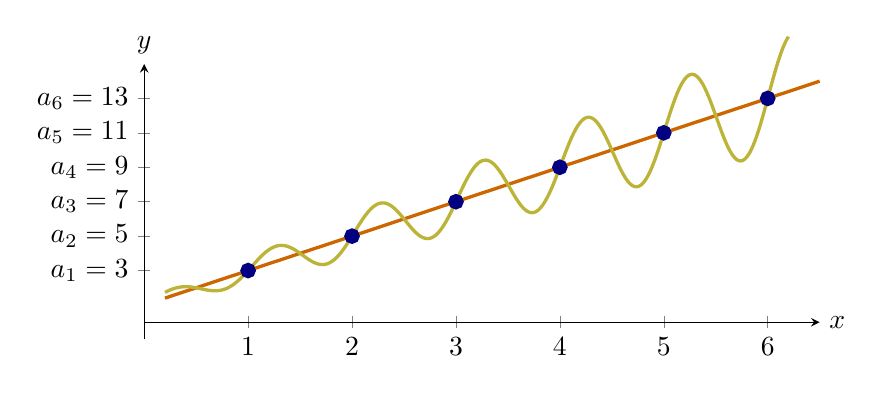
\begin{tikzpicture}
	\begin{axis}[
            domain=.8:6.5,xmin=0,xmax=6.5,ymin=-1,ymax=15,
            width=4in,
            height=2in,
            axis lines =middle, xlabel=$x$, ylabel=$y$,
            xtick={1,2,...,6},
            ytick={3,5,7,9,11,13},
            yticklabels={$a_1 = 3$,$a_2=5$,$a_3=7$,$a_4=9$,$a_5=11$,$a_6=13$},
            every axis y label/.style={at=(current axis.above origin),anchor=south},
            every axis x label/.style={at=(current axis.right of origin),anchor=west},
            clip=false,
            %axis on top,
          ]
       
           \addplot [penColor5,very thick,smooth,domain=.2:6.5]{2*x+1};
          \addplot [penColor6,very thick,smooth,domain=.2:6.2,samples=300]{(2*x+1)*(1+.25*sin(deg(2*pi*x)))};
          \addplot[color=penColor,fill=penColor,only marks,mark=*,ultra thick] coordinates{(1,3)};  %% closed hole        
          \addplot[color=penColor,fill=penColor,only marks,mark=*,ultra thick] coordinates{(2,5)};  %% closed hole        
          \addplot[color=penColor,fill=penColor,only marks,mark=*,ultra thick] coordinates{(3,7)};  %% closed hole        
          \addplot[color=penColor,fill=penColor,only marks,mark=*,ultra thick] coordinates{(4,9)};  %% closed hole        
          \addplot[color=penColor,fill=penColor,only marks,mark=*,ultra thick] coordinates{(5,11)};  %% closed hole    
          \addplot[color=penColor,fill=penColor,only marks,mark=*,ultra thick] coordinates{(6,13)};  %% closed hole         
        \end{axis}
\end{tikzpicture}
\end{image}

Let's see what happens if use a positive integer $n$ as an input for each function.

\begin{itemize}
\item Since $f(x) =  2x+1$, $f(n) = 2n+1$.
\item To evaluate $g(n)$, note that since $\sin(k \pi) = \answer[given]{0}$ for all integers $k$.  Thus, $g(n) = \frac{2n+1}{4}(4+\sin(n \pi)) = \frac{2n+1}{\cancel{4}}(\cancel{4}) = 2n+1$.
\end{itemize}

It should not be too surprising that several functions can be used to represent the same sequence because the sequence is defined only for integers, while the functions above are defined for \emph{all} real $x$-values in their domains. 
\end{example}

While there are many examples of sequences, there are two important types of sequences that arise in applications.
















\section*{Two important types of sequences}

\subsection*{Arithmetic sequences}

The first type of sequence we examine is an \textbf{\textcolor{purple!85!blue}{arithmetic sequence}}.  
%{Mathematically, the word \dfn{family}
%  does not have an entirely precise definition; a family of things is
%  a \dfn{collection} or a \dfn{set} of things, but family
%  also has a connotation of some sort of relatedness.} 

\begin{definition}  \textbf{\textcolor{green!50!black}{Arithmetic Sequence}} 


  An \textbf{arithmetic sequence} (sometimes called an arithmetic
  progression)\index{arithmetic progression} is a sequence for which the
  difference between subsequent elements is constant.
\end{definition}


\begin{example}
  Here is a representation of a certain arithmetic sequence.
  \begin{image}
  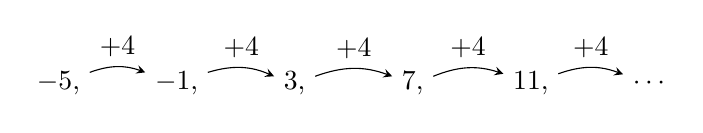
\begin{tikzpicture}[node distance=1.5cm]
    \node (a1) {$-5$,};
    \node (a2) [right of=a1] {$-1$,};
    \node (a3) [right of=a2] {$3$,};
    \node (a4) [right of=a3] {$7$,};
    \node (a5) [right of=a4] {$11$,};
    \node (a6) [right of=a5] {$\cdots$};

    \path[->] (a1) edge [bend left=20] node[above]{$+4$} (a2);
    \path[->] (a2) edge [bend left=20] node[above]{$+4$} (a3);
    \path[->] (a3) edge [bend left=20] node[above]{$+4$} (a4);
    \path[->] (a4) edge [bend left=20] node[above]{$+4$} (a5);
    \path[->] (a5) edge [bend left=20] node[above]{$+4$} (a6);
  \end{tikzpicture}
  \end{image}
  
 \begin{question}
 By looking at the plot above, which type of curve can be be used to model an arithmetic sequence?
  \wordChoice{    \choice[correct]{lines}     \choice{parabolas}     \choice{polynomials}     \choice{exponential curves} }

  \begin{feedback}
    Since the average growth rate of a line is constant regardless of
    the size of the interval chosen, arithmetic sequences correspond to
    lines.
  \end{feedback}
\end{question}


  By requiring that the starting index be $n_0=0$ for the sequence $\{a_n\}_{n=0}$, the terms in the sequence are given explicitly by the formula $a_n=\answer[given]{4n-5}$,
  or recursively by the rule $a_0 = \answer[given]{-5}$ and $a_{n+1} = a_n
  + \answer[given]{4}$. 

  The difference between subsequent elements in this sequence is always four.
\end{example}

In general, the terms in an arithmetic sequence $\{a_n\}_{n=0}$ in which subsequent terms differ
by $m$ can be written as
\[
a_n = m n + a_0.
\]
Alternatively, we could describe an arithmetic sequence recursively,
by giving a starting value $a_0$, and using the rule that $a_{n} =
a_{n-1} + m$.  You should check that this general statement holds for our 
two examples.


\begin{remark}
The arithmetic mean of two numbers $a$ and $b$ is defined to be $\frac{a+b}{2}$. Note that every term in an arithmetic sequence is the \textbf{arithmetic mean} of its two neighbors.  
\end{remark}

\subsection*{Plots of arithmetic sequences}

Recall that arithmetic sequences are those where the difference
between neighboring elements is constant.  Arithmetic sequences are
analogues of lines.  Consider the earlier example.





\begin{example}
\begin{image}
  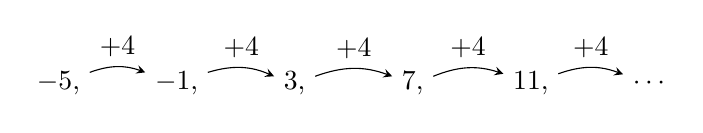
\begin{tikzpicture}[node distance=1.5cm]
    \node (a1) {$-5$,};
    \node (a2) [right of=a1] {$-1$,};
    \node (a3) [right of=a2] {$3$,};
    \node (a4) [right of=a3] {$7$,};
    \node (a5) [right of=a4] {$11$,};
    \node (a6) [right of=a5] {$\cdots$};
    
    \path[->] (a1) edge [bend left=20] node[above]{$+4$} (a2);
    \path[->] (a2) edge [bend left=20] node[above]{$+4$} (a3);
    \path[->] (a3) edge [bend left=20] node[above]{$+4$} (a4);
    \path[->] (a4) edge [bend left=20] node[above]{$+4$} (a5);
    \path[->] (a5) edge [bend left=20] node[above]{$+4$} (a6);
  \end{tikzpicture}
\end{image}

By requiring that the lower index of the sequence be $n_0=0$, we can check out a graph of the sequence.

\begin{image}
\begin{tikzpicture}
	\begin{axis}[
            domain=0:6,xmin=0,xmax=5,ymin=-9,ymax=15,
            width=4in,
            height=2in,
            axis lines =middle, xlabel=$n$, ylabel=$a$,
            xtick={1,2,...,4},
            ytick={-5,-1,...,11},
            yticklabels={$a_0 = -5$,$a_1=-1$,$a_2=3$,$a_3=7$,$a_4=11$},
            every axis y label/.style={at=(current axis.above origin),anchor=south},
            every axis x label/.style={at=(current axis.right of origin),anchor=west},
            clip=false,
            %axis on top,
          ]
          \addplot[color=penColor,fill=penColor,only marks,mark=*] coordinates{(0,-5)};  %% closed hole          
          \addplot[color=penColor,fill=penColor,only marks,mark=*] coordinates{(1,-1)};  %% closed hole          
          \addplot[color=penColor,fill=penColor,only marks,mark=*] coordinates{(2,3)};  %% closed hole          
          \addplot[color=penColor,fill=penColor,only marks,mark=*] coordinates{(3,7)};  %% closed hole          
          \addplot[color=penColor,fill=penColor,only marks,mark=*] coordinates{(4,11)};  %% closed hole  
        \end{axis}
\end{tikzpicture}
\end{image}

By noting that the explicit formula for the $n$-th term in this sequence is $a_n = 4n-5$, we can try to find a function of a real variable that coincides with this.  The simple rule of replacing $n$ with $x$ works here; we can set $f(x) = 4x-5$ and graph both on the same set of axes.

\begin{image}
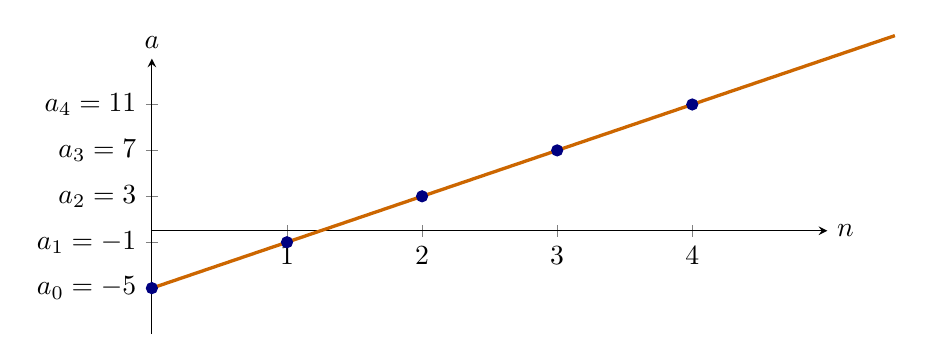
\begin{tikzpicture}
	\begin{axis}[
            domain=0:6,xmin=0,xmax=5,ymin=-9,ymax=15,
            width=4in,
            height=2in,
            axis lines =middle, xlabel=$n$, ylabel=$a$,
            xtick={1,2,...,4},
            ytick={-5,-1,...,11},
            yticklabels={$a_0 = -5$,$a_1=-1$,$a_2=3$,$a_3=7$,$a_4=11$},
            every axis y label/.style={at=(current axis.above origin),anchor=south},
            every axis x label/.style={at=(current axis.right of origin),anchor=west},
            clip=false,
            %axis on top,
          ]
                     \addplot [penColor5,very thick,smooth,domain=0:5.5]{4*x-5};
          \addplot[color=penColor,fill=penColor,only marks,mark=*] coordinates{(0,-5)};  %% closed hole          
          \addplot[color=penColor,fill=penColor,only marks,mark=*] coordinates{(1,-1)};  %% closed hole          
          \addplot[color=penColor,fill=penColor,only marks,mark=*] coordinates{(2,3)};  %% closed hole          
          \addplot[color=penColor,fill=penColor,only marks,mark=*] coordinates{(3,7)};  %% closed hole          
          \addplot[color=penColor,fill=penColor,only marks,mark=*] coordinates{(4,11)};  %% closed hole  
        \end{axis}
\end{tikzpicture}
\end{image}

We see that the common difference is actually the \wordChoice{\choice[correct]{slope}\choice{the $y$-coordinate of the $y$-intercept}} of the line.
\end{example}

\begin{example}
Here is an arithmetic sequence that decreases as its index increases.

\begin{image}
  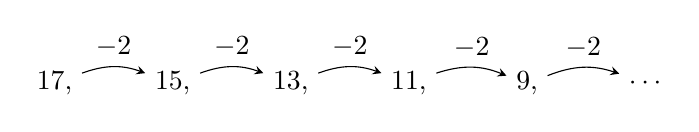
\begin{tikzpicture}[node distance=1.5cm]
    \node (a1) {$17$,};
    \node (a2) [right of=a1] {$15$,};
    \node (a3) [right of=a2] {$13$,};
    \node (a4) [right of=a3] {$11$,};
    \node (a5) [right of=a4] {$9$,};
    \node (a6) [right of=a5] {$\cdots$};

    \path[->] (a1) edge [bend left=20] node[above]{$-2$} (a2);
    \path[->] (a2) edge [bend left=20] node[above]{$-2$} (a3);
    \path[->] (a3) edge [bend left=20] node[above]{$-2$} (a4);
    \path[->] (a4) edge [bend left=20] node[above]{$-2$} (a5);
    \path[->] (a5) edge [bend left=20] node[above]{$-2$} (a6);
  \end{tikzpicture}
\end{image}

We can graph the terms.

\begin{image}
\begin{tikzpicture}
	\begin{axis}[
            domain=0:6,xmin=0,xmax=5,ymin=7,ymax=19,
            width=4in,
            height=2in,
            xtick={1,2,...,4},
            ytick={17,15,...,9},
            yticklabels={$a_0 = 17$,$a_1=15$,$a_2=13$,$a_3=11$,$a_4=9$},
            axis lines =middle, xlabel=$n$, ylabel=$a$,
            every axis y label/.style={at=(current axis.above origin),anchor=south},
            every axis x label/.style={at=(current axis.right of origin),anchor=west},
            clip=false,
            %axis on top,
          ]
          \addplot[color=penColor,fill=penColor,only marks,mark=*] coordinates{(0,17)};  %% closed hole          
          \addplot[color=penColor,fill=penColor,only marks,mark=*] coordinates{(1,15)};  %% closed hole          
          \addplot[color=penColor,fill=penColor,only marks,mark=*] coordinates{(2,13)};  %% closed hole          
          \addplot[color=penColor,fill=penColor,only marks,mark=*] coordinates{(3,11)};  %% closed hole          
          \addplot[color=penColor,fill=penColor,only marks,mark=*] coordinates{(4,9)};  %% closed hole  
        \end{axis}
\end{tikzpicture}
\end{image}

By setting $n_0=0$, we can find an explicit formula for the $n$-th term in the sequence; indeed $a_n = \answer[given]{-2n+17}$.  As such, we can easily find a function of a real variable $f(x)$ that coincides with the sequence on their common domains by replacing $n$ with $x$ to obtain $f(x) = \answer[given]{-2x+17}$.

We can graph both of these on the same set of axes.

\begin{image}
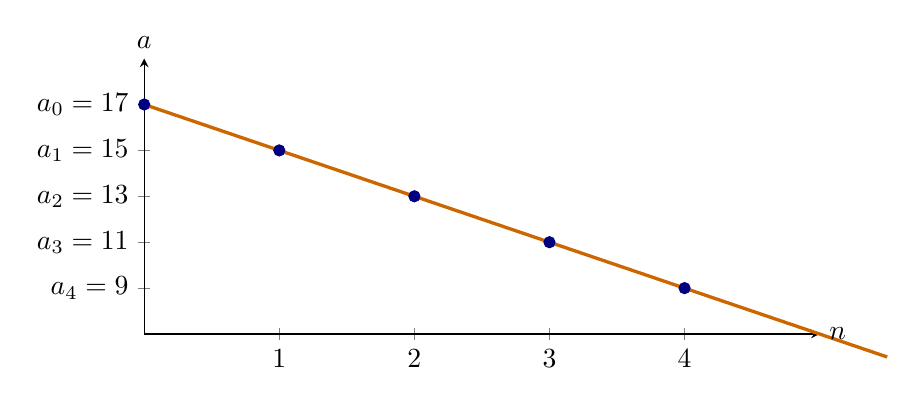
\begin{tikzpicture}
	\begin{axis}[
            domain=0:6,xmin=0,xmax=5,ymin=7,ymax=19,
            width=4in,
            height=2in,
            xtick={1,2,...,4},
            ytick={17,15,...,9},
            yticklabels={$a_0 = 17$,$a_1=15$,$a_2=13$,$a_3=11$,$a_4=9$},
            axis lines =middle, xlabel=$n$, ylabel=$a$,
            every axis y label/.style={at=(current axis.above origin),anchor=south},
            every axis x label/.style={at=(current axis.right of origin),anchor=west},
            clip=false,
            %axis on top,
          ]
          \addplot [penColor5,very thick,smooth,domain=0:5.5]{-2*x+17};
          \addplot[color=penColor,fill=penColor,only marks,mark=*] coordinates{(0,17)};  %% closed hole          
          \addplot[color=penColor,fill=penColor,only marks,mark=*] coordinates{(1,15)};  %% closed hole          
          \addplot[color=penColor,fill=penColor,only marks,mark=*] coordinates{(2,13)};  %% closed hole          
          \addplot[color=penColor,fill=penColor,only marks,mark=*] coordinates{(3,11)};  %% closed hole          
          \addplot[color=penColor,fill=penColor,only marks,mark=*] coordinates{(4,9)};  %% closed hole  
        \end{axis}
\end{tikzpicture}
\end{image}


\end{example}















\subsection*{Geometric sequences}

A second very important family of sequences we consider are geometric sequences.  

\begin{definition} \textbf{\textcolor{green!50!black}{Geometric Sequence}} 


  A \textbf{geometric sequence} (sometimes called a geometric
  progression)\index{geometric progression} is a sequence for which the
  ratio between subsequent elements is constant.
\end{definition}

\begin{example}
  Here is an example of a geometric sequence.
  \begin{image}
    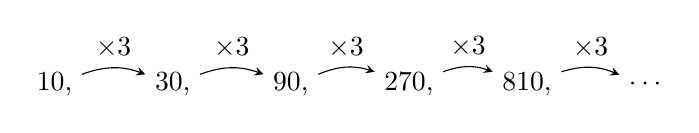
\begin{tikzpicture}[node distance=1.5cm]
    \node (a1) {$10$,};
    \node (a2) [right of=a1] {$30$,};
    \node (a3) [right of=a2] {$90$,};
    \node (a4) [right of=a3] {$270$,};
    \node (a5) [right of=a4] {$810$,};
    \node (a6) [right of=a5] {$\cdots$};

    \path[->] (a1) edge [bend left=20] node[above] {$\times 3$} (a2);
    \path[->] (a2) edge [bend left=20] node[above] {$\times 3$} (a3);
    \path[->] (a3) edge [bend left=20] node[above] {$\times 3$} (a4);
    \path[->] (a4) edge [bend left=20] node[above] {$\times 3$} (a5);
    \path[->] (a5) edge [bend left=20] node[above] {$\times 3$} (a6);
  \end{tikzpicture}
  \end{image}
By setting the initial index $n_0=0$ , the terms of this sequence can be given explicitly by the formula $a_n=\answer[given]{10\cdot
    3^{n}}$, or recursively by the rule $a_0 = \answer[given]{10}$ and
  $a_{n+1} = \answer[given]{3}\cdot a_n$. The ratio between any subsequent elements of our sequence is three.
\end{example}

A geometric sequence can also decrease as it progresses.

\begin{example}
  Here is an example of a geometric sequence.
  \begin{image}
    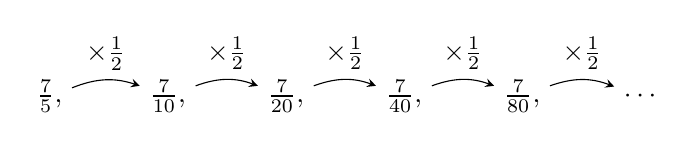
\begin{tikzpicture}[node distance=1.5cm]
    \node (a1) {$\frac{7}{5}$,};
    \node (a2) [right of=a1] {$\frac{7}{10}$,};
    \node (a3) [right of=a2] {$\frac{7}{20}$,};
    \node (a4) [right of=a3] {$\frac{7}{40}$,};
    \node (a5) [right of=a4] {$\frac{7}{80}$,};
    \node (a6) [right of=a5] {$\cdots$};

    \path[->] (a1) edge [bend left=20] node[above] {$\times\frac{1}{2}$} (a2);
    \path[->] (a2) edge [bend left=20] node[above] {$\times\frac{1}{2}$} (a3);
    \path[->] (a3) edge [bend left=20] node[above] {$\times\frac{1}{2}$} (a4);
    \path[->] (a4) edge [bend left=20] node[above] {$\times\frac{1}{2}$} (a5);
    \path[->] (a5) edge [bend left=20] node[above] {$\times\frac{1}{2}$} (a6);
  \end{tikzpicture}
  \end{image}
By setting the initial index $n_0=0$ , the terms in this sequence are given by the formula $a_n=\answer[given]{\left(\frac{7}{5}\right)\cdot
    \left(\frac{1}{2}\right)^{n}}$, or the recursive rule $a_0 = \answer[given]{\frac{7}{5}}$ and
  $a_{n+1} = \answer[given]{\left(\frac{1}{2}\right)}\cdot a_n$. The ratio between subsequent terms 
  of this sequence is always one half.
\end{example}

In general, a geometric sequence $\{a_n\}_{n=0}$ in which the ratio between
subsequent terms is $r$ can be written as
\[
a_n = a_0 \cdot r^{n}.
\]
Alternatively, we could describe a geometric sequence
recursively, by giving a starting value $a_0$, and using the rule that
$a_{n} = r \cdot a_{n-1}$.  As usual, you should check that these general 
rules hold for the specific examples we've considered.

\begin{remark}
The geometric mean of two numbers $a$ and $b$ is defined to be
$\sqrt{ab}$. Note that every term is the \textbf{geometric mean} of its two neighbors.   

%Of course, that raises another question: why is the geometric mean
%called \textit{geometric?}  One geometric interpretation of the
%geometric mean of $a$ and $b$ is this: the geometric mean is the side
%length of a square whose area is equal to that of the rectangle having
%side lengths $a$ and $b$.
\end{remark}
%


\subsection*{Plots of geometric sequences}

Let's look at plots of some of our special sequences.   

\begin{example}
Consider the previously illustrated example below.
\begin{image}
    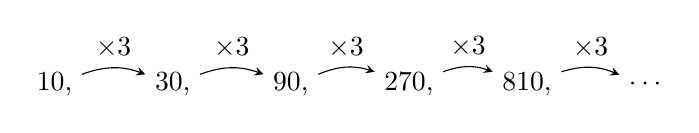
\begin{tikzpicture}[node distance=1.5cm]
    \node (a1) {$10$,};
    \node (a2) [right of=a1] {$30$,};
    \node (a3) [right of=a2] {$90$,};
    \node (a4) [right of=a3] {$270$,};
    \node (a5) [right of=a4] {$810$,};
    \node (a6) [right of=a5] {$\cdots$};

    \path[->] (a1) edge [bend left=20] node[above] {$\times 3$} (a2);
    \path[->] (a2) edge [bend left=20] node[above] {$\times 3$} (a3);
    \path[->] (a3) edge [bend left=20] node[above] {$\times 3$} (a4);
    \path[->] (a4) edge [bend left=20] node[above] {$\times 3$} (a5);
    \path[->] (a5) edge [bend left=20] node[above] {$\times 3$} (a6);
  \end{tikzpicture}
\end{image}
Let's plot the terms of the sequence. 
\begin{image}
\begin{tikzpicture}
	\begin{axis}[
            domain=0:6,xmin=0,xmax=5,ymin=-100,ymax=900,
            width=4in,
            height=2in,
            xtick={1,2,...,5},
            ytick={10,30,90,270,810},
            yticklabels={},%$a_1 = 10$,$a_2=30$,$a_3=90$,$a_4=270$,$a_5=810$},
            axis lines =middle, xlabel=$n$, ylabel=$a$,
            every axis y label/.style={at=(current axis.above origin),anchor=south},
            every axis x label/.style={at=(current axis.right of origin),anchor=west},
            clip=false,
            %axis on top,
          ]
          \addplot[color=penColor,fill=penColor,only marks,mark=*] coordinates{(0,10)};  %% closed hole          
          \addplot[color=penColor,fill=penColor,only marks,mark=*] coordinates{(1,30)};  %% closed hole          
          \addplot[color=penColor,fill=penColor,only marks,mark=*] coordinates{(2,90)};  %% closed hole          
          \addplot[color=penColor,fill=penColor,only marks,mark=*] coordinates{(3,270)};  %% closed hole          
          \addplot[color=penColor,fill=penColor,only marks,mark=*] coordinates{(4,810)};  %% closed hole  
        \end{axis}
\end{tikzpicture}
\end{image}

The formula for the terms in the sequence in this example was $a_n = 10 \cdot 3^n$. We can easily find a function of a real variable $f(x)$ that coincides with the sequence on their common domains by replacing $n$ with $x$ to obtain $f(x) = \answer[given]{10 \cdot 3^x}$ and graph them both on a common set of axes.


\begin{image}
\begin{tikzpicture}
	\begin{axis}[
            domain=0:6,xmin=0,xmax=5,ymin=-100,ymax=900,
            width=4in,
            height=2in,
            xtick={1,2,...,4},
            ytick={10,30,90,270,810},
            yticklabels={},%$a_1 = 10$,$a_2=30$,$a_3=90$,$a_4=270$,$a_5=810$},
            axis lines =middle, xlabel=$n$, ylabel=$a$,
            every axis y label/.style={at=(current axis.above origin),anchor=south},
            every axis x label/.style={at=(current axis.right of origin),anchor=west},
            clip=false,
            %axis on top,
          ]
	\addplot [penColor5,very thick,smooth,domain=0:4.1]{10*3^x};
          \addplot[color=penColor,fill=penColor,only marks,mark=*] coordinates{(0,10)};  %% closed hole          
          \addplot[color=penColor,fill=penColor,only marks,mark=*] coordinates{(1,30)};  %% closed hole          
          \addplot[color=penColor,fill=penColor,only marks,mark=*] coordinates{(2,90)};  %% closed hole          
          \addplot[color=penColor,fill=penColor,only marks,mark=*] coordinates{(3,270)};  %% closed hole          
          \addplot[color=penColor,fill=penColor,only marks,mark=*] coordinates{(4,810)};  %% closed hole  
        \end{axis}
\end{tikzpicture}
\end{image}
\end{example}

Now let's consider the second example of a geometric sequence from before, which is illustrated below.

%MAKE NOT CRAZY FRACTIONS%%%%%%%

\begin{image}
  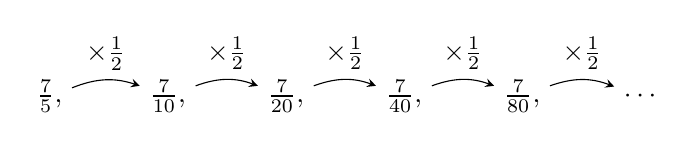
\begin{tikzpicture}[node distance=1.5cm]
    \node (a1) {$\frac{7}{5}$,};
    \node (a2) [right of=a1] {$\frac{7}{10}$,};
    \node (a3) [right of=a2] {$\frac{7}{20}$,};
    \node (a4) [right of=a3] {$\frac{7}{40}$,};
    \node (a5) [right of=a4] {$\frac{7}{80}$,};
    \node (a6) [right of=a5] {$\cdots$};
    
    \path[->] (a1) edge [bend left=20] node[above] {$\times\frac{1}{2}$} (a2);
    \path[->] (a2) edge [bend left=20] node[above] {$\times\frac{1}{2}$} (a3);
    \path[->] (a3) edge [bend left=20] node[above] {$\times\frac{1}{2}$} (a4);
    \path[->] (a4) edge [bend left=20] node[above] {$\times\frac{1}{2}$} (a5);
    \path[->] (a5) edge [bend left=20] node[above] {$\times\frac{1}{2}$} (a6);
  \end{tikzpicture}
\end{image}

In this example, the explicit formula the terms were given by the formula $a_n = \frac{7}{5} \cdot \left(\frac{1}{2}\right)^n$, so we can find a function of a real variable $f(x)$ that coincides with the sequence by setting $f(x) = \frac{7}{5} \cdot \left(\frac{1}{2}\right)^x$.  We can plot these on the same set of axes.

\begin{image}
\begin{tikzpicture}
	\begin{axis}[
            domain=0:6,xmin=0,xmax=5,ymin=0,ymax=2,
            width=4in,
            height=2in,
            xtick={1,2,...,4},
            ytick={1.4,.7,.35,.175,.0875},
            yticklabels={},%$a_1 = 10$,$a_2=30$,$a_3=90$,$a_4=270$,$a_5=810$},
            axis lines =middle, xlabel=$n$, ylabel=$a$,
            every axis y label/.style={at=(current axis.above origin),anchor=south},
            every axis x label/.style={at=(current axis.right of origin),anchor=west},
            clip=false,
            %axis on top,
          ]
	\addplot [penColor5,very thick,smooth,domain=0:4.9]{1.4*.5^x};          
          \addplot[color=penColor,fill=penColor,only marks,mark=*] coordinates{(0,7/5)};  %% closed hole          
          \addplot[color=penColor,fill=penColor,only marks,mark=*] coordinates{(1,7/10)};  %% closed hole          
          \addplot[color=penColor,fill=penColor,only marks,mark=*] coordinates{(2,7/20)};  %% closed hole          
          \addplot[color=penColor,fill=penColor,only marks,mark=*] coordinates{(3,7/40)};  %% closed hole          
          \addplot[color=penColor,fill=penColor,only marks,mark=*] coordinates{(4,7/80)};  %% closed hole  
        \end{axis}
\end{tikzpicture}
\end{image}

\begin{question}
  These examples illustrate an important fact.  If the common ratio between successive terms is greater than one, the geometric sequence will increase, but if it is between zero and one, the terms will decrease.    In each case, when the common ratio between successive elements of a geometric sequence is positive, which type of curves below model geometric sequences?
\wordChoice{    \choice{lines}    \choice{parabolas}    \choice{polynomials}    \choice[correct]{exponential curves}}

  \begin{feedback}
  If a geometric sequence is expressed as $a_n = a_1 \cdot r^{n-1}$,
  then in function notation we have $a(x) = a_1 \cdot r^{x-1}$, an
  exponential function.
  \end{feedback}
\end{question}

Can all geometric sequences be modeled using an exponential?  A third example explores this.  Consider the sequence modeled below.
\begin{image}
  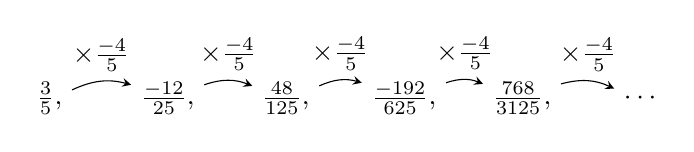
\begin{tikzpicture}[node distance=1.5cm]
    \node (a1) {$\frac{3}{5}$,};
    \node (a2) [right of=a1] {$\frac{-12}{25}$,};
    \node (a3) [right of=a2] {$\frac{48}{125}$,};
    \node (a4) [right of=a3] {$\frac{-192}{625}$,};L
    \node (a5) [right of=a4] {$\frac{768}{3125}$,};
    \node (a6) [right of=a5] {$\cdots$};
    
    \path[->] (a1) edge [bend left=20] node[above] {$\times\frac{-4}{5}$} (a2);
    \path[->] (a2) edge [bend left=20] node[above] {$\times\frac{-4}{5}$} (a3);
    \path[->] (a3) edge [bend left=20] node[above] {$\times\frac{-4}{5}$} (a4);
    \path[->] (a4) edge [bend left=20] node[above] {$\times\frac{-4}{5}$} (a5);
    \path[->] (a5) edge [bend left=20] node[above] {$\times\frac{-4}{5}$} (a6);
  \end{tikzpicture}
\end{image}
We can find a formula for the $n$-th term.  As before, setting the initial index as $n_0=0$, we can write $a_n = \frac{3}{5} \cdot \left( -\frac{4}{5}\right)^n$ and plot the terms.
\begin{image}
\begin{tikzpicture}
	\begin{axis}[
            domain=0:6,xmin=0,xmax=5,ymin=-.7,ymax=.7,
            width=4in,
            height=2in,
            xtick={1,2,...,4},
            ytick={.6,-.48,.384,-.3072,.24576},
            yticklabels={},%$a_1 = 10$,$a_2=30$,$a_3=90$,$a_4=270$,$a_5=810$},
            axis lines =middle, xlabel=$n$, ylabel=$a$,
            every axis y label/.style={at=(current axis.above origin),anchor=south},
            every axis x label/.style={at=(current axis.right of origin),anchor=west},
            clip=false,
            %axis on top,
          ]
          \addplot[color=penColor,fill=penColor,only marks,mark=*] coordinates{(0,3/5)};  %% closed hole          
          \addplot[color=penColor,fill=penColor,only marks,mark=*] coordinates{(1,-12/25)};  %% closed hole          
          \addplot[color=penColor,fill=penColor,only marks,mark=*] coordinates{(2,48/125)};  %% closed hole          
          \addplot[color=penColor,fill=penColor,only marks,mark=*] coordinates{(3,-192/625)};  %% closed hole          
          \addplot[color=penColor,fill=penColor,only marks,mark=*] coordinates{(4,768/3125)};  %% closed hole  
        \end{axis}
\end{tikzpicture}
\end{image}
The sign of this sequence alternates, so there is no exponential function of a real variable that will model this sequence.   However, we may note that

\[
a_n = \frac{3}{5} \cdot \left( -\frac{4}{5}\right)^n = \frac{3}{5} \cdot \left( - 1 \cdot \frac{4}{5}\right)^n =\frac{3}{5} \cdot (-1)^n \left(\frac{4}{5}\right)^n
\]

Replacing $(-1)^n$ with $\cos(\pi x)$ as we did in a previous example gives us a function \[f(x) = \frac{3}{5} \left(\frac{4}{5}\right)^x \cos(\pi x)\] that agrees with the sequence on their common domains.

Geometric sequences play an important role in the coming sections, so it is useful to have a good feel for what plots of these sequences do!

\begin{quote}
``Obvious" is the most dangerous word in mathematics" -E.T. Bell
\end{quote}


















\begin{center}
\textbf{\textcolor{green!50!black}{



\begin{center}
\textbf{\textcolor{green!50!black}{ooooo-=-=-=-ooOoo-=-=-=-ooooo}} \\

more examples can be found by following this link\\ \link[More Examples of Sequences]{https://ximera.osu.edu/csccmathematics/precalculus1/precalculus1/sequences/examples/exampleList}

\end{center}
}} \\

more examples can be found by following this link\\ \link[More Examples of Sequences]{https://ximera.osu.edu/csccmathematics/precalculus1/precalculus1/sequences/examples/exampleList}

\end{center}






\end{document}
